\ifdefined\COMPLETE
\else
    \input{./preambule-2010-utf8.ltx}
    \usepackage{alterqcm}
    \begin{document}
\fi

\ifdefined\CORRECTION
    \begin{alterqcm}[lq=10cm,correction]
\else
    \begin{alterqcm}[lq=10cm]
\fi



 \AQquestion[br=2]{Pour résoudre l'équation $\qquad 1-3x=8x+5$,\\
 on peut se ramener à la résolution de l'équation\ldots}{%
 {$-11x = -4$},
 {$11x = -4$},
 {$5x=6$}
 }
 

 \AQquestion[br=2]{Pour résoudre l'équation $ \qquad (2x-1)(2-3x)=0$,\\
  on peut se ramener à la résolution de l'équation\ldots}{%
 { on développe $(2x-1)(2-3x)=0$, },%
 {\begin{minipage}[t]{6cm} on résout chacune des équations $2x-1=0$ et $2-3x=0$,
    \end{minipage}},%
   {\begin{minipage}[t]{6cm} on divise chaque membre de l'équation par $2-3x$
  \end{minipage}}
 }
 
 
 \AQquestion[br=3]{Si $b>c$, alors\ldots}{%
   {\begin{minipage}[t]{6.5cm} on ne peut pas comparer $-2b$ et $-2c$, \end{minipage}},
 {$-2b > -2c$},
 {$-2b < -2c$}
 }
 
  
 \AQquestion[br=1]{Les solutions de l'inéquation $-2x \geqslant 4$}{%
    {\hbox {\raise -4.5mm \hbox{\begin{tikzpicture}[scale=.65]
         \tkzInit[xmin=-5,xmax=4,xstep=1]
         \tkzDrawX
         \tkzXHW     {-5/F//-2/T/] } % Hachures de -inf à -2
         \tkzText(0,-.6){\scriptsize $0$}  
         \tkzText(-2,-.6){\scriptsize $-2$}  
      \end{tikzpicture} }              
     }},
    {\hbox {\raise -4.5mm \hbox{ \begin{tikzpicture}[scale=.65]
         \tkzInit[xmin=-5,xmax=4,xstep=1]
         \tkzDrawX
         \tkzXHW     {-2/F/[/4/ } % Hachures de -inf à -2
         \tkzText(0,-.6){\scriptsize $0$}  
         \tkzText(-2,-.6){\scriptsize $-2$}  
      \end{tikzpicture}
    }}},                
    {\hbox {\raise -4.5mm \hbox{ \begin{tikzpicture}[scale=.65]
         \tkzInit[xmin=2,xmax=10,xstep=1]
         \tkzDrawX
         \tkzXHW     {6/F/[/10/ } % Hachures de -inf à -2
         \tkzText(2,-.6){\scriptsize $2$}  
         \tkzText(3,-.6){\scriptsize $3$}  
         \tkzText(6,-.6){\scriptsize $6$}  
      \end{tikzpicture}                 
     }}}
 }
 
 \AQquestion[br=3]{Les solutions de l'inéquation $-3x \geqslant 0$, sont les nombres\ldots}{%
   {$x \geqslant 0$},
 {$x \geqslant 3$},
 {$x \leqslant 0$}
 }


 \AQquestion[br=3]{Pour résoudre l'équation $2-5x>-2x+1$,
 on peut se ramener à la résolution de l'équation\ldots}{%
 {$1>-7x$},
 {$-3x<1$},
 {$3x<1$}
 }


 \AQquestion[br=1]{« Julie a 15 ans et son père a 42 ans. Dans combien d'années l'âge de son père sera égal au double de l'âge de Julie ? » \\
 Pour résoudre ce problème, il faut commencer par}{%
 {préciser l'inconnue choisie,},
 {écrire une équation,},
 {résoudre une équation.}
 }
 
\end{alterqcm}

\ifdefined\COMPLETE
\else
    \end{document}
\fi